% Options for packages loaded elsewhere
\PassOptionsToPackage{unicode}{hyperref}
\PassOptionsToPackage{hyphens}{url}
%
\documentclass[
]{article}
\usepackage{lmodern}
\usepackage{amssymb,amsmath}
\usepackage{ifxetex,ifluatex}
\ifnum 0\ifxetex 1\fi\ifluatex 1\fi=0 % if pdftex
  \usepackage[T1]{fontenc}
  \usepackage[utf8]{inputenc}
  \usepackage{textcomp} % provide euro and other symbols
\else % if luatex or xetex
  \usepackage{unicode-math}
  \defaultfontfeatures{Scale=MatchLowercase}
  \defaultfontfeatures[\rmfamily]{Ligatures=TeX,Scale=1}
\fi
% Use upquote if available, for straight quotes in verbatim environments
\IfFileExists{upquote.sty}{\usepackage{upquote}}{}
\IfFileExists{microtype.sty}{% use microtype if available
  \usepackage[]{microtype}
  \UseMicrotypeSet[protrusion]{basicmath} % disable protrusion for tt fonts
}{}
\makeatletter
\@ifundefined{KOMAClassName}{% if non-KOMA class
  \IfFileExists{parskip.sty}{%
    \usepackage{parskip}
  }{% else
    \setlength{\parindent}{0pt}
    \setlength{\parskip}{6pt plus 2pt minus 1pt}}
}{% if KOMA class
  \KOMAoptions{parskip=half}}
\makeatother
\usepackage{xcolor}
\IfFileExists{xurl.sty}{\usepackage{xurl}}{} % add URL line breaks if available
\IfFileExists{bookmark.sty}{\usepackage{bookmark}}{\usepackage{hyperref}}
\hypersetup{
  pdftitle={A reference feature based method for quantification and identification of LC-MS based untargeted metabolomics},
  pdfauthor={luanenhui},
  hidelinks,
  pdfcreator={LaTeX via pandoc}}
\urlstyle{same} % disable monospaced font for URLs
\usepackage[margin=1in]{geometry}
\usepackage{color}
\usepackage{fancyvrb}
\newcommand{\VerbBar}{|}
\newcommand{\VERB}{\Verb[commandchars=\\\{\}]}
\DefineVerbatimEnvironment{Highlighting}{Verbatim}{commandchars=\\\{\}}
% Add ',fontsize=\small' for more characters per line
\usepackage{framed}
\definecolor{shadecolor}{RGB}{248,248,248}
\newenvironment{Shaded}{\begin{snugshade}}{\end{snugshade}}
\newcommand{\AlertTok}[1]{\textcolor[rgb]{0.94,0.16,0.16}{#1}}
\newcommand{\AnnotationTok}[1]{\textcolor[rgb]{0.56,0.35,0.01}{\textbf{\textit{#1}}}}
\newcommand{\AttributeTok}[1]{\textcolor[rgb]{0.77,0.63,0.00}{#1}}
\newcommand{\BaseNTok}[1]{\textcolor[rgb]{0.00,0.00,0.81}{#1}}
\newcommand{\BuiltInTok}[1]{#1}
\newcommand{\CharTok}[1]{\textcolor[rgb]{0.31,0.60,0.02}{#1}}
\newcommand{\CommentTok}[1]{\textcolor[rgb]{0.56,0.35,0.01}{\textit{#1}}}
\newcommand{\CommentVarTok}[1]{\textcolor[rgb]{0.56,0.35,0.01}{\textbf{\textit{#1}}}}
\newcommand{\ConstantTok}[1]{\textcolor[rgb]{0.00,0.00,0.00}{#1}}
\newcommand{\ControlFlowTok}[1]{\textcolor[rgb]{0.13,0.29,0.53}{\textbf{#1}}}
\newcommand{\DataTypeTok}[1]{\textcolor[rgb]{0.13,0.29,0.53}{#1}}
\newcommand{\DecValTok}[1]{\textcolor[rgb]{0.00,0.00,0.81}{#1}}
\newcommand{\DocumentationTok}[1]{\textcolor[rgb]{0.56,0.35,0.01}{\textbf{\textit{#1}}}}
\newcommand{\ErrorTok}[1]{\textcolor[rgb]{0.64,0.00,0.00}{\textbf{#1}}}
\newcommand{\ExtensionTok}[1]{#1}
\newcommand{\FloatTok}[1]{\textcolor[rgb]{0.00,0.00,0.81}{#1}}
\newcommand{\FunctionTok}[1]{\textcolor[rgb]{0.00,0.00,0.00}{#1}}
\newcommand{\ImportTok}[1]{#1}
\newcommand{\InformationTok}[1]{\textcolor[rgb]{0.56,0.35,0.01}{\textbf{\textit{#1}}}}
\newcommand{\KeywordTok}[1]{\textcolor[rgb]{0.13,0.29,0.53}{\textbf{#1}}}
\newcommand{\NormalTok}[1]{#1}
\newcommand{\OperatorTok}[1]{\textcolor[rgb]{0.81,0.36,0.00}{\textbf{#1}}}
\newcommand{\OtherTok}[1]{\textcolor[rgb]{0.56,0.35,0.01}{#1}}
\newcommand{\PreprocessorTok}[1]{\textcolor[rgb]{0.56,0.35,0.01}{\textit{#1}}}
\newcommand{\RegionMarkerTok}[1]{#1}
\newcommand{\SpecialCharTok}[1]{\textcolor[rgb]{0.00,0.00,0.00}{#1}}
\newcommand{\SpecialStringTok}[1]{\textcolor[rgb]{0.31,0.60,0.02}{#1}}
\newcommand{\StringTok}[1]{\textcolor[rgb]{0.31,0.60,0.02}{#1}}
\newcommand{\VariableTok}[1]{\textcolor[rgb]{0.00,0.00,0.00}{#1}}
\newcommand{\VerbatimStringTok}[1]{\textcolor[rgb]{0.31,0.60,0.02}{#1}}
\newcommand{\WarningTok}[1]{\textcolor[rgb]{0.56,0.35,0.01}{\textbf{\textit{#1}}}}
\usepackage{graphicx,grffile}
\makeatletter
\def\maxwidth{\ifdim\Gin@nat@width>\linewidth\linewidth\else\Gin@nat@width\fi}
\def\maxheight{\ifdim\Gin@nat@height>\textheight\textheight\else\Gin@nat@height\fi}
\makeatother
% Scale images if necessary, so that they will not overflow the page
% margins by default, and it is still possible to overwrite the defaults
% using explicit options in \includegraphics[width, height, ...]{}
\setkeys{Gin}{width=\maxwidth,height=\maxheight,keepaspectratio}
% Set default figure placement to htbp
\makeatletter
\def\fps@figure{htbp}
\makeatother
\setlength{\emergencystretch}{3em} % prevent overfull lines
\providecommand{\tightlist}{%
  \setlength{\itemsep}{0pt}\setlength{\parskip}{0pt}}
\setcounter{secnumdepth}{-\maxdimen} % remove section numbering

\title{A reference feature based method for quantification and identification
of LC-MS based untargeted metabolomics}
\author{luanenhui}
\date{2020-03-05}

\begin{document}
\maketitle

\hypertarget{introduction}{%
\subsection{Introduction}\label{introduction}}

RFQI is a LC-MS/MS based untargeted metabolomics analysis pipeline.

\hypertarget{module}{%
\subsection{Module}\label{module}}

\begin{enumerate}
\def\labelenumi{\arabic{enumi}.}
\item
  build reference feature table
\item
  Mapping MS2 to reference feature table
\item
  Build MS2 similarity distribution
\item
  Idenfification
\item
  Quantification
\end{enumerate}

\hypertarget{build-reference-feature-table}{%
\subsubsection{build reference feature
table}\label{build-reference-feature-table}}

\begin{Shaded}
\begin{Highlighting}[]
\KeywordTok{library}\NormalTok{(RFQI)}
\KeywordTok{options}\NormalTok{(}\DataTypeTok{stringsAsFactors =} \OtherTok{FALSE}\NormalTok{)}
\end{Highlighting}
\end{Shaded}

First, we need to build a reference a feature table using a set of mzxml
files.

\begin{Shaded}
\begin{Highlighting}[]
\NormalTok{files <-}\StringTok{ }\KeywordTok{dir}\NormalTok{(}\KeywordTok{system.file}\NormalTok{(}\DataTypeTok{package=}\StringTok{"RFQI"}\NormalTok{, }\DataTypeTok{dir=}\StringTok{"extdata"}\NormalTok{), }
              \DataTypeTok{full.name=}\OtherTok{TRUE}\NormalTok{, }
              \DataTypeTok{pattern=}\StringTok{"mzXML$"}\NormalTok{)}
\NormalTok{param =}\StringTok{ }\KeywordTok{new}\NormalTok{(}\StringTok{"ParamSet"}\NormalTok{, }\DataTypeTok{binSize=}\FloatTok{0.25}\NormalTok{, }\DataTypeTok{peakwidth=}\KeywordTok{c}\NormalTok{(}\DecValTok{2}\NormalTok{,}\DecValTok{30}\NormalTok{), }\DataTypeTok{ppm=}\DecValTok{10}\NormalTok{, }\DataTypeTok{noise=}\DecValTok{0}\NormalTok{, }\DataTypeTok{absMz=}\FloatTok{0.005}\NormalTok{, }\DataTypeTok{absRt=}\DecValTok{15}\NormalTok{)}
\end{Highlighting}
\end{Shaded}

We also need to set a reference mzXML

\begin{Shaded}
\begin{Highlighting}[]
\NormalTok{refFile =}\StringTok{ }\NormalTok{files[}\DecValTok{1}\NormalTok{]}
\NormalTok{files =}\StringTok{ }\NormalTok{files[}\DecValTok{2}\NormalTok{]}
\end{Highlighting}
\end{Shaded}

Then we extract peaks from mzXML files and group them. This step is
time-consuming, we can save the result for later use

\begin{Shaded}
\begin{Highlighting}[]
\NormalTok{features =}\StringTok{ }\KeywordTok{getPeakRange_multipleFiles}\NormalTok{(}\DataTypeTok{f.in =}\NormalTok{ files, }\DataTypeTok{ref =}\NormalTok{ refFile, }\DataTypeTok{param=}\NormalTok{param, }\DataTypeTok{cores=}\DecValTok{2}\NormalTok{)}
\CommentTok{#> [1] "beginning to get peaks from each sample"}
\CommentTok{#> [1] "beginning to group/combine peaks"}
\CommentTok{#> [1] "group 9157 peaks divided into 37 part cost 0.145906333128611 minutes"}
\CommentTok{#> [1] "group 6466 peaks divided into 1 part cost 0.73112698396047 minutes"}
\CommentTok{# save(features, ref, files, file="test_features.rData")}
\end{Highlighting}
\end{Shaded}

features is a list, containing two data frame. Peaks are original peaks
extracted from mzXML files by centwave, group\_FT are features by
combing adjacent peaks.

\begin{Shaded}
\begin{Highlighting}[]
\KeywordTok{str}\NormalTok{(features, }\DataTypeTok{max.level =} \DecValTok{1}\NormalTok{)}
\CommentTok{#> List of 2}
\CommentTok{#>  $ group_FT: chr [1:6437, 1:14] "70.509233166622" "72.0439013574296" "72.0808839267337" "74.0571356829619" ...}
\CommentTok{#>   ..- attr(*, "dimnames")=List of 2}
\CommentTok{#>  $ peaks   : num [1:9157, 1:13] 162 275 503 577 99 ...}
\CommentTok{#>   ..- attr(*, "dimnames")=List of 2}
\end{Highlighting}
\end{Shaded}

We have generate a features, so you can simply load it into R enviroment

\begin{Shaded}
\begin{Highlighting}[]
\CommentTok{# data("features", package="RFQI")}
\end{Highlighting}
\end{Shaded}

\hypertarget{mapping-ms2-to-a-reference-feature-table}{%
\subsubsection{Mapping MS2 to a reference feature
table}\label{mapping-ms2-to-a-reference-feature-table}}

\emph{After extracting features from MS1 spectrum, we need to mapping
MS2 spectrum to features for annotating.}

First, we need extract MS2 spectrum from mzXML files. These files can be
files used for constructing feature table, also can be other files, as
soon as they are generated in the same enviroment (e.g.~same tissue
type, same LC-MS/MS parameter)

getMS2FromFiles function receive mzXML files as input, and output a
list.

\begin{Shaded}
\begin{Highlighting}[]
\NormalTok{files <-}\StringTok{ }\KeywordTok{dir}\NormalTok{(}\KeywordTok{system.file}\NormalTok{(}\DataTypeTok{package=}\StringTok{"RFQI"}\NormalTok{, }\DataTypeTok{dir=}\StringTok{"extdata"}\NormalTok{), }\DataTypeTok{full.name=}\OtherTok{TRUE}\NormalTok{, }\DataTypeTok{pattern=}\StringTok{"mzXML$"}\NormalTok{)}
\NormalTok{MS2 =}\StringTok{ }\KeywordTok{getMS2FromFiles}\NormalTok{(}\DataTypeTok{files=}\NormalTok{files, }\DataTypeTok{ref_file =}\NormalTok{ refFile)}
\KeywordTok{str}\NormalTok{(MS2, }\DataTypeTok{max.level =} \DecValTok{1}\NormalTok{)}
\CommentTok{#> List of 2}
\CommentTok{#>  $ MS2          :List of 6858}
\CommentTok{#>  $ precursorInfo:'data.frame':   6858 obs. of  6 variables:}
\end{Highlighting}
\end{Shaded}

Before we map MS2 to features, we can filter out some MS2

\begin{Shaded}
\begin{Highlighting}[]
\NormalTok{mzCount =}\StringTok{ }\KeywordTok{unlist}\NormalTok{(}\KeywordTok{lapply}\NormalTok{(MS2}\OperatorTok{$}\NormalTok{MS2, nrow)) }\CommentTok{# A qualified MS2 spectrum should have at least 3 fragments}
\NormalTok{mzMaxInt =}\StringTok{ }\KeywordTok{unlist}\NormalTok{(}\KeywordTok{lapply}\NormalTok{(MS2}\OperatorTok{$}\NormalTok{MS2, }\ControlFlowTok{function}\NormalTok{(x)\{}\KeywordTok{max}\NormalTok{(x[,}\DecValTok{2}\NormalTok{])\}))  }\CommentTok{# A qualified MS2 spectrum should have at least one fragment whose intensity greater than 32 (user defined)}
\NormalTok{CountFlag =}\StringTok{ }\OperatorTok{!}\NormalTok{(mzCount }\OperatorTok\StringTok{ }\KeywordTok{c}\NormalTok{(}\DecValTok{0}\NormalTok{,}\DecValTok{1}\NormalTok{,}\DecValTok{2}\NormalTok{))}
\NormalTok{IntFlag =}\StringTok{ }\NormalTok{mzMaxInt }\OperatorTok{>}\StringTok{ }\DecValTok{50}
\NormalTok{flag =}\StringTok{ }\NormalTok{CountFlag }\OperatorTok{&}\StringTok{ }\NormalTok{IntFlag}

\NormalTok{MS2}\OperatorTok{$}\NormalTok{MS2 =}\StringTok{ }\NormalTok{MS2}\OperatorTok{$}\NormalTok{MS2[flag]}
\NormalTok{MS2}\OperatorTok{$}\NormalTok{precursorInfo =}\StringTok{ }\NormalTok{MS2}\OperatorTok{$}\NormalTok{precursorInfo[flag,]}
\end{Highlighting}
\end{Shaded}

We also need set names for each MS2

\begin{Shaded}
\begin{Highlighting}[]
\KeywordTok{names}\NormalTok{(MS2}\OperatorTok{$}\NormalTok{MS2) =}\StringTok{ }\KeywordTok{rownames}\NormalTok{(MS2}\OperatorTok{$}\NormalTok{precursorInfo) =}\StringTok{ }\KeywordTok{sapply}\NormalTok{(}\DecValTok{1}\OperatorTok{:}\KeywordTok{nrow}\NormalTok{(MS2}\OperatorTok{$}\NormalTok{precursorInfo),}
\NormalTok{convert_num_to_char, }\DataTypeTok{prefix =} \StringTok{"M"}\NormalTok{, }\DataTypeTok{n=}\KeywordTok{nchar}\NormalTok{(}\KeywordTok{nrow}\NormalTok{(MS2}\OperatorTok{$}\NormalTok{precursorInfo)))}
\end{Highlighting}
\end{Shaded}

Next, we align MS2 to feature based on precursor's m/z and rt.

\begin{Shaded}
\begin{Highlighting}[]
\NormalTok{db.MS2 =}\StringTok{ }\KeywordTok{align_MS2_to_MS1}\NormalTok{(}\DataTypeTok{ms2Info =}\NormalTok{ MS2, }\DataTypeTok{features =}\NormalTok{ features)}
\end{Highlighting}
\end{Shaded}

\hypertarget{build-ms2-similarity-distribution}{%
\subsubsection{Build MS2 similarity
distribution}\label{build-ms2-similarity-distribution}}

\begin{itemize}
\tightlist
\item
  RFQI use multiple MS2 to identify one feature. First, we need to build
  an MS2 similarity distribution using MS2 belonging to the same feature
  *
\end{itemize}

Next, we calculate MS2 similarity matrix belonging to same feature The
time complexity is O(n2), where n represents the number of MS2 belonging
the the same feature, we can limit the max number using maxMS2 parameter

\begin{Shaded}
\begin{Highlighting}[]
\CommentTok{# we can calcalate similarity distribution for one feature}
\NormalTok{idx =}\StringTok{ }\KeywordTok{getFeatureHasMS2}\NormalTok{(}\DataTypeTok{MS2DB=}\NormalTok{db.MS2, }\DataTypeTok{n=}\DecValTok{2}\NormalTok{)  }\CommentTok{# n is the minimum number of MS2 belonging to the same feature}
\NormalTok{distri =}\StringTok{ }\KeywordTok{get_ms2Cor_inner}\NormalTok{(}\DataTypeTok{MS2DB =}\NormalTok{ db.MS2, }\DataTypeTok{cores=}\DecValTok{2}\NormalTok{, }\DataTypeTok{maxMS2 =} \DecValTok{100}\NormalTok{, }\DataTypeTok{idx=}\NormalTok{idx[}\DecValTok{1}\NormalTok{])}
\end{Highlighting}
\end{Shaded}

\begin{Shaded}
\begin{Highlighting}[]
\KeywordTok{plot}\NormalTok{(}\KeywordTok{density}\NormalTok{(distri[[}\DecValTok{1}\NormalTok{]][,}\DecValTok{1}\NormalTok{], }\DataTypeTok{na.rm=}\OtherTok{TRUE}\NormalTok{), }\DataTypeTok{main=}\StringTok{"MS2 similarity distribution"}\NormalTok{, }\DataTypeTok{col=}\StringTok{"red"}\NormalTok{, }\DataTypeTok{xlab=}\StringTok{"cosine similarity score"}\NormalTok{)}
\ControlFlowTok{for}\NormalTok{ (i }\ControlFlowTok{in} \DecValTok{2}\OperatorTok{:}\KeywordTok{nrow}\NormalTok{(distri[[}\DecValTok{1}\NormalTok{]]))\{}
  \KeywordTok{lines}\NormalTok{(}\KeywordTok{density}\NormalTok{(distri[[}\DecValTok{1}\NormalTok{]][,i], }\DataTypeTok{na.rm=}\OtherTok{TRUE}\NormalTok{), }\DataTypeTok{col=}\StringTok{"red"}\NormalTok{)}
\NormalTok{\}}
\end{Highlighting}
\end{Shaded}

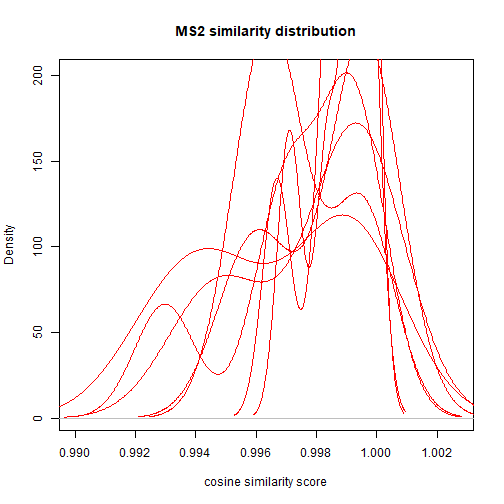
\includegraphics{tutorial_files/figure-latex/unnamed-chunk-12-1.pdf}

If we do not appoint feature ID, get\_ms2Cor\_inner() will compute
similarity matrix for all features having minimum MS2

\begin{Shaded}
\begin{Highlighting}[]
\NormalTok{db.MS2.subset =}\StringTok{ }\KeywordTok{list}\NormalTok{(}\DataTypeTok{MS2=}\NormalTok{db.MS2}\OperatorTok{$}\NormalTok{MS2[}\DecValTok{1}\OperatorTok{:}\DecValTok{500}\NormalTok{], }\DataTypeTok{MS2_to_MS1=}\NormalTok{db.MS2}\OperatorTok{$}\NormalTok{MS2_to_MS1[}\DecValTok{1}\OperatorTok{:}\DecValTok{500}\NormalTok{,]) }\CommentTok{# this line is only for test}
\NormalTok{ms2InnerCor =}\StringTok{ }\KeywordTok{get_ms2Cor_inner}\NormalTok{(}\DataTypeTok{MS2DB =}\NormalTok{ db.MS2.subset,}\DataTypeTok{cores =} \DecValTok{2}\NormalTok{, }\DataTypeTok{n=}\DecValTok{2}\NormalTok{, }\DataTypeTok{maxMS2 =} \DecValTok{100}\NormalTok{)}
\end{Highlighting}
\end{Shaded}

\hypertarget{identification}{%
\subsubsection{Identification}\label{identification}}

Now, we can identify features. Identification is based on existing
standard metabolites MS2 spectrum. We have offer a standard MS2 spectrum
database.

\begin{Shaded}
\begin{Highlighting}[]
\KeywordTok{data}\NormalTok{(}\StringTok{"spectrumDB"}\NormalTok{, }\DataTypeTok{package =} \StringTok{"RFQI"}\NormalTok{)}
\KeywordTok{str}\NormalTok{(spectrumDB, }\DataTypeTok{max.level =} \DecValTok{1}\NormalTok{)}
\CommentTok{#> List of 2}
\CommentTok{#>  $ spectrum:List of 3}
\CommentTok{#>  $ Info    : chr [1:3, 1:5] "HMDB0000267" "HMDB0000641" "HMDB0000148" "L-Pyroglutamic acid" ...}
\CommentTok{#>   ..- attr(*, "dimnames")=List of 2}
\end{Highlighting}
\end{Shaded}

First, we need match features' m/z and standar metabolites m/z. As
metabolites have multiple possible adduct when ionization, we need
appoint the liquidChromatography column type and ESI mode (i.e, positive
or negative). RFQI has offer a list of adduct corresponding to each
colum-mode, so you just need to set adduct=``RP\_pos'', etc.

\begin{Shaded}
\begin{Highlighting}[]
\KeywordTok{print}\NormalTok{(}\StringTok{"beginning identify"}\NormalTok{)}
\CommentTok{#> [1] "beginning identify"}
\NormalTok{anno =}\StringTok{ }\KeywordTok{get_identify}\NormalTok{(}\DataTypeTok{lib =}\NormalTok{ spectrumDB, }\DataTypeTok{MS2DB =}\NormalTok{ db.MS2.subset, }\DataTypeTok{MS2_inner_cor =}\NormalTok{ ms2InnerCor, }\DataTypeTok{absMz =} \FloatTok{0.045}\NormalTok{, }\DataTypeTok{adduct=}\StringTok{"RP_pos"}\NormalTok{, }\DataTypeTok{cores=}\DecValTok{3}\NormalTok{)}
\CommentTok{#>         ScoreMedian ScoreMax ScoreSD FDRFilter num_pros num_cons ratio labid}
\CommentTok{#> FT00017          NA       NA      NA        NA       NA       NA    NA    NA}
\CommentTok{#> FT00077          NA       NA      NA        NA       NA       NA    NA    NA}
\CommentTok{#> FT00136          NA       NA      NA        NA       NA       NA    NA    NA}
\CommentTok{#> FT00152          NA       NA      NA        NA       NA       NA    NA    NA}
\CommentTok{#> FT00312          NA       NA      NA        NA       NA       NA    NA    NA}
\CommentTok{#> FT00313          NA       NA      NA        NA       NA       NA    NA    NA}
\CommentTok{#> FT00315          NA       NA      NA        NA       NA       NA    NA    NA}
\CommentTok{#> FT00336          NA       NA      NA        NA       NA       NA    NA    NA}
\CommentTok{#> FT00395          NA       NA      NA        NA       NA       NA    NA    NA}
\CommentTok{#> FT00449          NA       NA      NA        NA       NA       NA    NA    NA}
\CommentTok{#> FT00465          NA       NA      NA        NA       NA       NA    NA    NA}
\CommentTok{#> FT00470          NA       NA      NA        NA       NA       NA    NA    NA}
\CommentTok{#> FT00487          NA       NA      NA        NA       NA       NA    NA    NA}
\CommentTok{#> FT00491          NA       NA      NA        NA       NA       NA    NA    NA}
\CommentTok{#> FT00546          NA       NA      NA        NA       NA       NA    NA    NA}
\CommentTok{#> FT00591          NA       NA      NA        NA       NA       NA    NA    NA}
\CommentTok{#> FT00596          NA       NA      NA        NA       NA       NA    NA    NA}
\CommentTok{#> FT00607          NA       NA      NA        NA       NA       NA    NA    NA}
\CommentTok{#> FT00636          NA       NA      NA        NA       NA       NA    NA    NA}
\CommentTok{#> FT00713          NA       NA      NA        NA       NA       NA    NA    NA}
\CommentTok{#> FT00761          NA       NA      NA        NA       NA       NA    NA    NA}
\CommentTok{#> FT00856          NA       NA      NA        NA       NA       NA    NA    NA}
\CommentTok{#> FT00872          NA       NA      NA        NA       NA       NA    NA    NA}
\CommentTok{#> FT00951          NA       NA      NA        NA       NA       NA    NA    NA}
\CommentTok{#> FT01031          NA       NA      NA        NA       NA       NA    NA    NA}
\CommentTok{#> FT01060          NA       NA      NA        NA       NA       NA    NA    NA}
\CommentTok{#> FT01131          NA       NA      NA        NA       NA       NA    NA    NA}
\CommentTok{#> FT01152          NA       NA      NA        NA       NA       NA    NA    NA}
\CommentTok{#> FT01244          NA       NA      NA        NA       NA       NA    NA    NA}
\CommentTok{#> FT01329          NA       NA      NA        NA       NA       NA    NA    NA}
\CommentTok{#> FT01411          NA       NA      NA        NA       NA       NA    NA    NA}
\CommentTok{#> FT01429          NA       NA      NA        NA       NA       NA    NA    NA}
\CommentTok{#> FT01485          NA       NA      NA        NA       NA       NA    NA    NA}
\CommentTok{#> FT01501          NA       NA      NA        NA       NA       NA    NA    NA}
\CommentTok{#> FT01530          NA       NA      NA        NA       NA       NA    NA    NA}
\CommentTok{#> FT01596          NA       NA      NA        NA       NA       NA    NA    NA}
\CommentTok{#> FT01753          NA       NA      NA        NA       NA       NA    NA    NA}
\CommentTok{#> FT01782          NA       NA      NA        NA       NA       NA    NA    NA}
\CommentTok{#> FT01885          NA       NA      NA        NA       NA       NA    NA    NA}
\CommentTok{#> FT02067          NA       NA      NA        NA       NA       NA    NA    NA}
\CommentTok{#> FT02072          NA       NA      NA        NA       NA       NA    NA    NA}
\CommentTok{#> FT02111          NA       NA      NA        NA       NA       NA    NA    NA}
\CommentTok{#> FT02128          NA       NA      NA        NA       NA       NA    NA    NA}
\CommentTok{#> FT02144          NA       NA      NA        NA       NA       NA    NA    NA}
\CommentTok{#> FT02453          NA       NA      NA        NA       NA       NA    NA    NA}
\CommentTok{#> FT02478          NA       NA      NA        NA       NA       NA    NA    NA}
\CommentTok{#> FT02528          NA       NA      NA        NA       NA       NA    NA    NA}
\CommentTok{#> FT02739          NA       NA      NA        NA       NA       NA    NA    NA}
\CommentTok{#> FT02863          NA       NA      NA        NA       NA       NA    NA    NA}
\CommentTok{#> FT03052          NA       NA      NA        NA       NA       NA    NA    NA}
\CommentTok{#> FT03053          NA       NA      NA        NA       NA       NA    NA    NA}
\CommentTok{#> FT03060          NA       NA      NA        NA       NA       NA    NA    NA}
\CommentTok{#> FT03115          NA       NA      NA        NA       NA       NA    NA    NA}
\CommentTok{#> FT03386          NA       NA      NA        NA       NA       NA    NA    NA}
\CommentTok{#> FT03489          NA       NA      NA        NA       NA       NA    NA    NA}
\CommentTok{#> FT03619          NA       NA      NA        NA       NA       NA    NA    NA}
\CommentTok{#> FT03622          NA       NA      NA        NA       NA       NA    NA    NA}
\CommentTok{#> FT03713          NA       NA      NA        NA       NA       NA    NA    NA}
\CommentTok{#> FT03813          NA       NA      NA        NA       NA       NA    NA    NA}
\CommentTok{#> FT04032          NA       NA      NA        NA       NA       NA    NA    NA}
\CommentTok{#> FT04084          NA       NA      NA        NA       NA       NA    NA    NA}
\CommentTok{#> FT04197          NA       NA      NA        NA       NA       NA    NA    NA}
\CommentTok{#> FT04435          NA       NA      NA        NA       NA       NA    NA    NA}
\CommentTok{#> FT04564          NA       NA      NA        NA       NA       NA    NA    NA}
\CommentTok{#> FT04906          NA       NA      NA        NA       NA       NA    NA    NA}
\CommentTok{#> FT04959          NA       NA      NA        NA       NA       NA    NA    NA}
\CommentTok{#> FT04965          NA       NA      NA        NA       NA       NA    NA    NA}
\CommentTok{#> FT04976          NA       NA      NA        NA       NA       NA    NA    NA}
\CommentTok{#> FT05241          NA       NA      NA        NA       NA       NA    NA    NA}
\CommentTok{#> FT05324          NA       NA      NA        NA       NA       NA    NA    NA}
\CommentTok{#> FT05416          NA       NA      NA        NA       NA       NA    NA    NA}
\CommentTok{#> FT05436          NA       NA      NA        NA       NA       NA    NA    NA}
\CommentTok{#> FT05648          NA       NA      NA        NA       NA       NA    NA    NA}
\CommentTok{#> FT05913          NA       NA      NA        NA       NA       NA    NA    NA}
\CommentTok{#>         adduct}
\CommentTok{#> FT00017     NA}
\CommentTok{#> FT00077     NA}
\CommentTok{#> FT00136     NA}
\CommentTok{#> FT00152     NA}
\CommentTok{#> FT00312     NA}
\CommentTok{#> FT00313     NA}
\CommentTok{#> FT00315     NA}
\CommentTok{#> FT00336     NA}
\CommentTok{#> FT00395     NA}
\CommentTok{#> FT00449     NA}
\CommentTok{#> FT00465     NA}
\CommentTok{#> FT00470     NA}
\CommentTok{#> FT00487     NA}
\CommentTok{#> FT00491     NA}
\CommentTok{#> FT00546     NA}
\CommentTok{#> FT00591     NA}
\CommentTok{#> FT00596     NA}
\CommentTok{#> FT00607     NA}
\CommentTok{#> FT00636     NA}
\CommentTok{#> FT00713     NA}
\CommentTok{#> FT00761     NA}
\CommentTok{#> FT00856     NA}
\CommentTok{#> FT00872     NA}
\CommentTok{#> FT00951     NA}
\CommentTok{#> FT01031     NA}
\CommentTok{#> FT01060     NA}
\CommentTok{#> FT01131     NA}
\CommentTok{#> FT01152     NA}
\CommentTok{#> FT01244     NA}
\CommentTok{#> FT01329     NA}
\CommentTok{#> FT01411     NA}
\CommentTok{#> FT01429     NA}
\CommentTok{#> FT01485     NA}
\CommentTok{#> FT01501     NA}
\CommentTok{#> FT01530     NA}
\CommentTok{#> FT01596     NA}
\CommentTok{#> FT01753     NA}
\CommentTok{#> FT01782     NA}
\CommentTok{#> FT01885     NA}
\CommentTok{#> FT02067     NA}
\CommentTok{#> FT02072     NA}
\CommentTok{#> FT02111     NA}
\CommentTok{#> FT02128     NA}
\CommentTok{#> FT02144     NA}
\CommentTok{#> FT02453     NA}
\CommentTok{#> FT02478     NA}
\CommentTok{#> FT02528     NA}
\CommentTok{#> FT02739     NA}
\CommentTok{#> FT02863     NA}
\CommentTok{#> FT03052     NA}
\CommentTok{#> FT03053     NA}
\CommentTok{#> FT03060     NA}
\CommentTok{#> FT03115     NA}
\CommentTok{#> FT03386     NA}
\CommentTok{#> FT03489     NA}
\CommentTok{#> FT03619     NA}
\CommentTok{#> FT03622     NA}
\CommentTok{#> FT03713     NA}
\CommentTok{#> FT03813     NA}
\CommentTok{#> FT04032     NA}
\CommentTok{#> FT04084     NA}
\CommentTok{#> FT04197     NA}
\CommentTok{#> FT04435     NA}
\CommentTok{#> FT04564     NA}
\CommentTok{#> FT04906     NA}
\CommentTok{#> FT04959     NA}
\CommentTok{#> FT04965     NA}
\CommentTok{#> FT04976     NA}
\CommentTok{#> FT05241     NA}
\CommentTok{#> FT05324     NA}
\CommentTok{#> FT05416     NA}
\CommentTok{#> FT05436     NA}
\CommentTok{#> FT05648     NA}
\CommentTok{#> FT05913     NA}
\CommentTok{#> $FT00017}
\CommentTok{#> $FT00017$score}
\CommentTok{#> NULL}
\CommentTok{#> }
\CommentTok{#> $FT00017$adduct}
\CommentTok{#> character(0)}
\CommentTok{#> }
\CommentTok{#> }
\CommentTok{#> $FT00077}
\CommentTok{#> $FT00077$score}
\CommentTok{#> NULL}
\CommentTok{#> }
\CommentTok{#> $FT00077$adduct}
\CommentTok{#> character(0)}
\CommentTok{#> }
\CommentTok{#> }
\CommentTok{#> $FT00136}
\CommentTok{#> $FT00136$score}
\CommentTok{#> NULL}
\CommentTok{#> }
\CommentTok{#> $FT00136$adduct}
\CommentTok{#> character(0)}
\CommentTok{#> }
\CommentTok{#> }
\CommentTok{#> $FT00152}
\CommentTok{#> $FT00152$score}
\CommentTok{#> NULL}
\CommentTok{#> }
\CommentTok{#> $FT00152$adduct}
\CommentTok{#> character(0)}
\CommentTok{#> }
\CommentTok{#> }
\CommentTok{#> $FT00312}
\CommentTok{#> $FT00312$score}
\CommentTok{#> NULL}
\CommentTok{#> }
\CommentTok{#> $FT00312$adduct}
\CommentTok{#> character(0)}
\CommentTok{#> }
\CommentTok{#> }
\CommentTok{#> $FT00313}
\CommentTok{#> $FT00313$score}
\CommentTok{#> NULL}
\CommentTok{#> }
\CommentTok{#> $FT00313$adduct}
\CommentTok{#> character(0)}
\CommentTok{#> }
\CommentTok{#> }
\CommentTok{#> $FT00315}
\CommentTok{#> $FT00315$score}
\CommentTok{#> NULL}
\CommentTok{#> }
\CommentTok{#> $FT00315$adduct}
\CommentTok{#> character(0)}
\CommentTok{#> }
\CommentTok{#> }
\CommentTok{#> $FT00336}
\CommentTok{#> $FT00336$score}
\CommentTok{#> NULL}
\CommentTok{#> }
\CommentTok{#> $FT00336$adduct}
\CommentTok{#> character(0)}
\CommentTok{#> }
\CommentTok{#> }
\CommentTok{#> $FT00395}
\CommentTok{#> $FT00395$score}
\CommentTok{#> NULL}
\CommentTok{#> }
\CommentTok{#> $FT00395$adduct}
\CommentTok{#> character(0)}
\CommentTok{#> }
\CommentTok{#> }
\CommentTok{#> $FT00449}
\CommentTok{#> $FT00449$score}
\CommentTok{#> NULL}
\CommentTok{#> }
\CommentTok{#> $FT00449$adduct}
\CommentTok{#> character(0)}
\CommentTok{#> }
\CommentTok{#> }
\CommentTok{#> $FT00465}
\CommentTok{#> $FT00465$score}
\CommentTok{#> NULL}
\CommentTok{#> }
\CommentTok{#> $FT00465$adduct}
\CommentTok{#> character(0)}
\CommentTok{#> }
\CommentTok{#> }
\CommentTok{#> $FT00470}
\CommentTok{#> $FT00470$score}
\CommentTok{#> NULL}
\CommentTok{#> }
\CommentTok{#> $FT00470$adduct}
\CommentTok{#> character(0)}
\CommentTok{#> }
\CommentTok{#> }
\CommentTok{#> $FT00487}
\CommentTok{#> $FT00487$score}
\CommentTok{#> NULL}
\CommentTok{#> }
\CommentTok{#> $FT00487$adduct}
\CommentTok{#> character(0)}
\CommentTok{#> }
\CommentTok{#> }
\CommentTok{#> $FT00491}
\CommentTok{#> $FT00491$score}
\CommentTok{#> NULL}
\CommentTok{#> }
\CommentTok{#> $FT00491$adduct}
\CommentTok{#> character(0)}
\CommentTok{#> }
\CommentTok{#> }
\CommentTok{#> $FT00546}
\CommentTok{#> $FT00546$score}
\CommentTok{#> NULL}
\CommentTok{#> }
\CommentTok{#> $FT00546$adduct}
\CommentTok{#> character(0)}
\CommentTok{#> }
\CommentTok{#> }
\CommentTok{#> $FT00591}
\CommentTok{#> $FT00591$score}
\CommentTok{#> NULL}
\CommentTok{#> }
\CommentTok{#> $FT00591$adduct}
\CommentTok{#> character(0)}
\CommentTok{#> }
\CommentTok{#> }
\CommentTok{#> $FT00596}
\CommentTok{#> $FT00596$score}
\CommentTok{#> NULL}
\CommentTok{#> }
\CommentTok{#> $FT00596$adduct}
\CommentTok{#> character(0)}
\CommentTok{#> }
\CommentTok{#> }
\CommentTok{#> $FT00607}
\CommentTok{#> $FT00607$score}
\CommentTok{#> NULL}
\CommentTok{#> }
\CommentTok{#> $FT00607$adduct}
\CommentTok{#> character(0)}
\CommentTok{#> }
\CommentTok{#> }
\CommentTok{#> $FT00636}
\CommentTok{#> $FT00636$score}
\CommentTok{#> NULL}
\CommentTok{#> }
\CommentTok{#> $FT00636$adduct}
\CommentTok{#> character(0)}
\CommentTok{#> }
\CommentTok{#> }
\CommentTok{#> $FT00713}
\CommentTok{#> $FT00713$score}
\CommentTok{#>       HMDB0000148}
\CommentTok{#> M0221  0.00240861}
\CommentTok{#> }
\CommentTok{#> $FT00713$adduct}
\CommentTok{#> [1] "(M+HCOO+2H)+"}
\CommentTok{#> }
\CommentTok{#> }
\CommentTok{#> $FT00761}
\CommentTok{#> $FT00761$score}
\CommentTok{#> NULL}
\CommentTok{#> }
\CommentTok{#> $FT00761$adduct}
\CommentTok{#> character(0)}
\CommentTok{#> }
\CommentTok{#> }
\CommentTok{#> $FT00856}
\CommentTok{#> $FT00856$score}
\CommentTok{#>       HMDB0000267}
\CommentTok{#> M0445  0.04104061}
\CommentTok{#> }
\CommentTok{#> $FT00856$adduct}
\CommentTok{#> [1] "(M-H+2K)+"}
\CommentTok{#> }
\CommentTok{#> }
\CommentTok{#> $FT00872}
\CommentTok{#> $FT00872$score}
\CommentTok{#> NULL}
\CommentTok{#> }
\CommentTok{#> $FT00872$adduct}
\CommentTok{#> character(0)}
\CommentTok{#> }
\CommentTok{#> }
\CommentTok{#> $FT00951}
\CommentTok{#> $FT00951$score}
\CommentTok{#> NULL}
\CommentTok{#> }
\CommentTok{#> $FT00951$adduct}
\CommentTok{#> character(0)}
\CommentTok{#> }
\CommentTok{#> }
\CommentTok{#> $FT01031}
\CommentTok{#> $FT01031$score}
\CommentTok{#> NULL}
\CommentTok{#> }
\CommentTok{#> $FT01031$adduct}
\CommentTok{#> character(0)}
\CommentTok{#> }
\CommentTok{#> }
\CommentTok{#> $FT01060}
\CommentTok{#> $FT01060$score}
\CommentTok{#> NULL}
\CommentTok{#> }
\CommentTok{#> $FT01060$adduct}
\CommentTok{#> character(0)}
\CommentTok{#> }
\CommentTok{#> }
\CommentTok{#> $FT01131}
\CommentTok{#> $FT01131$score}
\CommentTok{#> NULL}
\CommentTok{#> }
\CommentTok{#> $FT01131$adduct}
\CommentTok{#> character(0)}
\CommentTok{#> }
\CommentTok{#> }
\CommentTok{#> $FT01152}
\CommentTok{#> $FT01152$score}
\CommentTok{#> NULL}
\CommentTok{#> }
\CommentTok{#> $FT01152$adduct}
\CommentTok{#> character(0)}
\CommentTok{#> }
\CommentTok{#> }
\CommentTok{#> $FT01244}
\CommentTok{#> $FT01244$score}
\CommentTok{#> NULL}
\CommentTok{#> }
\CommentTok{#> $FT01244$adduct}
\CommentTok{#> character(0)}
\CommentTok{#> }
\CommentTok{#> }
\CommentTok{#> $FT01329}
\CommentTok{#> $FT01329$score}
\CommentTok{#> NULL}
\CommentTok{#> }
\CommentTok{#> $FT01329$adduct}
\CommentTok{#> character(0)}
\CommentTok{#> }
\CommentTok{#> }
\CommentTok{#> $FT01411}
\CommentTok{#> $FT01411$score}
\CommentTok{#> NULL}
\CommentTok{#> }
\CommentTok{#> $FT01411$adduct}
\CommentTok{#> character(0)}
\CommentTok{#> }
\CommentTok{#> }
\CommentTok{#> $FT01429}
\CommentTok{#> $FT01429$score}
\CommentTok{#> NULL}
\CommentTok{#> }
\CommentTok{#> $FT01429$adduct}
\CommentTok{#> character(0)}
\CommentTok{#> }
\CommentTok{#> }
\CommentTok{#> $FT01485}
\CommentTok{#> $FT01485$score}
\CommentTok{#> NULL}
\CommentTok{#> }
\CommentTok{#> $FT01485$adduct}
\CommentTok{#> character(0)}
\CommentTok{#> }
\CommentTok{#> }
\CommentTok{#> $FT01501}
\CommentTok{#> $FT01501$score}
\CommentTok{#> NULL}
\CommentTok{#> }
\CommentTok{#> $FT01501$adduct}
\CommentTok{#> character(0)}
\CommentTok{#> }
\CommentTok{#> }
\CommentTok{#> $FT01530}
\CommentTok{#> $FT01530$score}
\CommentTok{#> NULL}
\CommentTok{#> }
\CommentTok{#> $FT01530$adduct}
\CommentTok{#> character(0)}
\CommentTok{#> }
\CommentTok{#> }
\CommentTok{#> $FT01596}
\CommentTok{#> $FT01596$score}
\CommentTok{#> NULL}
\CommentTok{#> }
\CommentTok{#> $FT01596$adduct}
\CommentTok{#> character(0)}
\CommentTok{#> }
\CommentTok{#> }
\CommentTok{#> $FT01753}
\CommentTok{#> $FT01753$score}
\CommentTok{#> NULL}
\CommentTok{#> }
\CommentTok{#> $FT01753$adduct}
\CommentTok{#> character(0)}
\CommentTok{#> }
\CommentTok{#> }
\CommentTok{#> $FT01782}
\CommentTok{#> $FT01782$score}
\CommentTok{#> NULL}
\CommentTok{#> }
\CommentTok{#> $FT01782$adduct}
\CommentTok{#> character(0)}
\CommentTok{#> }
\CommentTok{#> }
\CommentTok{#> $FT01885}
\CommentTok{#> $FT01885$score}
\CommentTok{#> NULL}
\CommentTok{#> }
\CommentTok{#> $FT01885$adduct}
\CommentTok{#> character(0)}
\CommentTok{#> }
\CommentTok{#> }
\CommentTok{#> $FT02067}
\CommentTok{#> $FT02067$score}
\CommentTok{#> NULL}
\CommentTok{#> }
\CommentTok{#> $FT02067$adduct}
\CommentTok{#> character(0)}
\CommentTok{#> }
\CommentTok{#> }
\CommentTok{#> $FT02072}
\CommentTok{#> $FT02072$score}
\CommentTok{#> NULL}
\CommentTok{#> }
\CommentTok{#> $FT02072$adduct}
\CommentTok{#> character(0)}
\CommentTok{#> }
\CommentTok{#> }
\CommentTok{#> $FT02111}
\CommentTok{#> $FT02111$score}
\CommentTok{#> NULL}
\CommentTok{#> }
\CommentTok{#> $FT02111$adduct}
\CommentTok{#> character(0)}
\CommentTok{#> }
\CommentTok{#> }
\CommentTok{#> $FT02128}
\CommentTok{#> $FT02128$score}
\CommentTok{#> NULL}
\CommentTok{#> }
\CommentTok{#> $FT02128$adduct}
\CommentTok{#> character(0)}
\CommentTok{#> }
\CommentTok{#> }
\CommentTok{#> $FT02144}
\CommentTok{#> $FT02144$score}
\CommentTok{#> NULL}
\CommentTok{#> }
\CommentTok{#> $FT02144$adduct}
\CommentTok{#> character(0)}
\CommentTok{#> }
\CommentTok{#> }
\CommentTok{#> $FT02453}
\CommentTok{#> $FT02453$score}
\CommentTok{#> NULL}
\CommentTok{#> }
\CommentTok{#> $FT02453$adduct}
\CommentTok{#> character(0)}
\CommentTok{#> }
\CommentTok{#> }
\CommentTok{#> $FT02478}
\CommentTok{#> $FT02478$score}
\CommentTok{#> NULL}
\CommentTok{#> }
\CommentTok{#> $FT02478$adduct}
\CommentTok{#> character(0)}
\CommentTok{#> }
\CommentTok{#> }
\CommentTok{#> $FT02528}
\CommentTok{#> $FT02528$score}
\CommentTok{#> NULL}
\CommentTok{#> }
\CommentTok{#> $FT02528$adduct}
\CommentTok{#> character(0)}
\CommentTok{#> }
\CommentTok{#> }
\CommentTok{#> $FT02739}
\CommentTok{#> $FT02739$score}
\CommentTok{#> NULL}
\CommentTok{#> }
\CommentTok{#> $FT02739$adduct}
\CommentTok{#> character(0)}
\CommentTok{#> }
\CommentTok{#> }
\CommentTok{#> $FT02863}
\CommentTok{#> $FT02863$score}
\CommentTok{#> NULL}
\CommentTok{#> }
\CommentTok{#> $FT02863$adduct}
\CommentTok{#> character(0)}
\CommentTok{#> }
\CommentTok{#> }
\CommentTok{#> $FT03052}
\CommentTok{#> $FT03052$score}
\CommentTok{#> NULL}
\CommentTok{#> }
\CommentTok{#> $FT03052$adduct}
\CommentTok{#> character(0)}
\CommentTok{#> }
\CommentTok{#> }
\CommentTok{#> $FT03053}
\CommentTok{#> $FT03053$score}
\CommentTok{#> NULL}
\CommentTok{#> }
\CommentTok{#> $FT03053$adduct}
\CommentTok{#> character(0)}
\CommentTok{#> }
\CommentTok{#> }
\CommentTok{#> $FT03060}
\CommentTok{#> $FT03060$score}
\CommentTok{#> NULL}
\CommentTok{#> }
\CommentTok{#> $FT03060$adduct}
\CommentTok{#> character(0)}
\CommentTok{#> }
\CommentTok{#> }
\CommentTok{#> $FT03115}
\CommentTok{#> $FT03115$score}
\CommentTok{#> NULL}
\CommentTok{#> }
\CommentTok{#> $FT03115$adduct}
\CommentTok{#> character(0)}
\CommentTok{#> }
\CommentTok{#> }
\CommentTok{#> $FT03386}
\CommentTok{#> $FT03386$score}
\CommentTok{#> NULL}
\CommentTok{#> }
\CommentTok{#> $FT03386$adduct}
\CommentTok{#> character(0)}
\CommentTok{#> }
\CommentTok{#> }
\CommentTok{#> $FT03489}
\CommentTok{#> $FT03489$score}
\CommentTok{#> NULL}
\CommentTok{#> }
\CommentTok{#> $FT03489$adduct}
\CommentTok{#> character(0)}
\CommentTok{#> }
\CommentTok{#> }
\CommentTok{#> $FT03619}
\CommentTok{#> $FT03619$score}
\CommentTok{#> NULL}
\CommentTok{#> }
\CommentTok{#> $FT03619$adduct}
\CommentTok{#> character(0)}
\CommentTok{#> }
\CommentTok{#> }
\CommentTok{#> $FT03622}
\CommentTok{#> $FT03622$score}
\CommentTok{#> NULL}
\CommentTok{#> }
\CommentTok{#> $FT03622$adduct}
\CommentTok{#> character(0)}
\CommentTok{#> }
\CommentTok{#> }
\CommentTok{#> $FT03713}
\CommentTok{#> $FT03713$score}
\CommentTok{#> NULL}
\CommentTok{#> }
\CommentTok{#> $FT03713$adduct}
\CommentTok{#> character(0)}
\CommentTok{#> }
\CommentTok{#> }
\CommentTok{#> $FT03813}
\CommentTok{#> $FT03813$score}
\CommentTok{#> NULL}
\CommentTok{#> }
\CommentTok{#> $FT03813$adduct}
\CommentTok{#> character(0)}
\CommentTok{#> }
\CommentTok{#> }
\CommentTok{#> $FT04032}
\CommentTok{#> $FT04032$score}
\CommentTok{#> NULL}
\CommentTok{#> }
\CommentTok{#> $FT04032$adduct}
\CommentTok{#> character(0)}
\CommentTok{#> }
\CommentTok{#> }
\CommentTok{#> $FT04084}
\CommentTok{#> $FT04084$score}
\CommentTok{#> NULL}
\CommentTok{#> }
\CommentTok{#> $FT04084$adduct}
\CommentTok{#> character(0)}
\CommentTok{#> }
\CommentTok{#> }
\CommentTok{#> $FT04197}
\CommentTok{#> $FT04197$score}
\CommentTok{#> NULL}
\CommentTok{#> }
\CommentTok{#> $FT04197$adduct}
\CommentTok{#> character(0)}
\CommentTok{#> }
\CommentTok{#> }
\CommentTok{#> $FT04435}
\CommentTok{#> $FT04435$score}
\CommentTok{#> NULL}
\CommentTok{#> }
\CommentTok{#> $FT04435$adduct}
\CommentTok{#> character(0)}
\CommentTok{#> }
\CommentTok{#> }
\CommentTok{#> $FT04564}
\CommentTok{#> $FT04564$score}
\CommentTok{#> NULL}
\CommentTok{#> }
\CommentTok{#> $FT04564$adduct}
\CommentTok{#> character(0)}
\CommentTok{#> }
\CommentTok{#> }
\CommentTok{#> $FT04906}
\CommentTok{#> $FT04906$score}
\CommentTok{#> NULL}
\CommentTok{#> }
\CommentTok{#> $FT04906$adduct}
\CommentTok{#> character(0)}
\CommentTok{#> }
\CommentTok{#> }
\CommentTok{#> $FT04959}
\CommentTok{#> $FT04959$score}
\CommentTok{#> NULL}
\CommentTok{#> }
\CommentTok{#> $FT04959$adduct}
\CommentTok{#> character(0)}
\CommentTok{#> }
\CommentTok{#> }
\CommentTok{#> $FT04965}
\CommentTok{#> $FT04965$score}
\CommentTok{#> NULL}
\CommentTok{#> }
\CommentTok{#> $FT04965$adduct}
\CommentTok{#> character(0)}
\CommentTok{#> }
\CommentTok{#> }
\CommentTok{#> $FT04976}
\CommentTok{#> $FT04976$score}
\CommentTok{#> NULL}
\CommentTok{#> }
\CommentTok{#> $FT04976$adduct}
\CommentTok{#> character(0)}
\CommentTok{#> }
\CommentTok{#> }
\CommentTok{#> $FT05241}
\CommentTok{#> $FT05241$score}
\CommentTok{#> NULL}
\CommentTok{#> }
\CommentTok{#> $FT05241$adduct}
\CommentTok{#> character(0)}
\CommentTok{#> }
\CommentTok{#> }
\CommentTok{#> $FT05324}
\CommentTok{#> $FT05324$score}
\CommentTok{#> NULL}
\CommentTok{#> }
\CommentTok{#> $FT05324$adduct}
\CommentTok{#> character(0)}
\CommentTok{#> }
\CommentTok{#> }
\CommentTok{#> $FT05416}
\CommentTok{#> $FT05416$score}
\CommentTok{#> NULL}
\CommentTok{#> }
\CommentTok{#> $FT05416$adduct}
\CommentTok{#> character(0)}
\CommentTok{#> }
\CommentTok{#> }
\CommentTok{#> $FT05436}
\CommentTok{#> $FT05436$score}
\CommentTok{#> NULL}
\CommentTok{#> }
\CommentTok{#> $FT05436$adduct}
\CommentTok{#> character(0)}
\CommentTok{#> }
\CommentTok{#> }
\CommentTok{#> $FT05648}
\CommentTok{#> $FT05648$score}
\CommentTok{#> NULL}
\CommentTok{#> }
\CommentTok{#> $FT05648$adduct}
\CommentTok{#> character(0)}
\CommentTok{#> }
\CommentTok{#> }
\CommentTok{#> $FT05913}
\CommentTok{#> $FT05913$score}
\CommentTok{#> NULL}
\CommentTok{#> }
\CommentTok{#> $FT05913$adduct}
\CommentTok{#> character(0)}
\KeywordTok{str}\NormalTok{(anno, }\DataTypeTok{max.level =} \DecValTok{1}\NormalTok{)}
\CommentTok{#> List of 2}
\CommentTok{#>  $ anno : logi[0 , 1:10] }
\CommentTok{#>   ..- attr(*, "dimnames")=List of 2}
\CommentTok{#>  $ score:List of 74}
\KeywordTok{print}\NormalTok{(}\StringTok{"end identify"}\NormalTok{)}
\CommentTok{#> [1] "end identify"}
\end{Highlighting}
\end{Shaded}

\hypertarget{quantification}{%
\subsubsection{Quantification}\label{quantification}}

We have build a reference feature table, and using MS2 to annotate it.
All we need to do for following mzXML files is quantify according to
feature table.

\begin{Shaded}
\begin{Highlighting}[]
\NormalTok{result =}\StringTok{ }\KeywordTok{list}\NormalTok{()}
\ControlFlowTok{for}\NormalTok{ (file }\ControlFlowTok{in}\NormalTok{ files)\{}
\NormalTok{  result[[file]] =}\StringTok{ }\KeywordTok{getPeaks_L}\NormalTok{(}\DataTypeTok{file =}\NormalTok{ file, }\DataTypeTok{peak_range =}\NormalTok{ features}\OperatorTok{$}\NormalTok{group_FT, }\DataTypeTok{ref_file =}\NormalTok{ refFile, }\DataTypeTok{MS1=}\OtherTok{TRUE}\NormalTok{, }\DataTypeTok{step=}\FloatTok{0.1}\NormalTok{, }\DataTypeTok{MS2=}\OtherTok{FALSE}\NormalTok{) }\CommentTok{# $peaks[,"into",drop=FA]}
\NormalTok{\}}
\CommentTok{#> method:  bin }
\CommentTok{#> step:  0.1 }
\CommentTok{#> method:  bin }
\CommentTok{#> step:  0.1 }
\CommentTok{#> method:  bin }
\CommentTok{#> step:  0.1}
\NormalTok{intensity =}\StringTok{ }\KeywordTok{do.call}\NormalTok{(cbind,result)}
\KeywordTok{colnames}\NormalTok{(intensity) =}\StringTok{ }\KeywordTok{names}\NormalTok{(result)}
\KeywordTok{str}\NormalTok{(intensity, }\DataTypeTok{max.level =} \DecValTok{1}\NormalTok{)}
\CommentTok{#> List of 12}
\CommentTok{#>  $ : num [1:6437, 1:9] 70.5 72 72.1 74.1 74.1 ...}
\CommentTok{#>   ..- attr(*, "dimnames")=List of 2}
\CommentTok{#>  $ : logi NA}
\CommentTok{#>  $ : logi NA}
\CommentTok{#>  $ :'data.frame':    3041 obs. of  3 variables:}
\CommentTok{#>  $ : num [1:6437, 1:9] 70.5 72 72.1 74.1 74.1 ...}
\CommentTok{#>   ..- attr(*, "dimnames")=List of 2}
\CommentTok{#>  $ : logi NA}
\CommentTok{#>  $ : logi NA}
\CommentTok{#>  $ :'data.frame':    6141 obs. of  3 variables:}
\CommentTok{#>  $ : num [1:6437, 1:9] 70.5 72 72.1 74.1 74.1 ...}
\CommentTok{#>   ..- attr(*, "dimnames")=List of 2}
\CommentTok{#>  $ : logi NA}
\CommentTok{#>  $ : logi NA}
\CommentTok{#>  $ :'data.frame':    6132 obs. of  3 variables:}
\CommentTok{#>  - attr(*, "dim")= int [1:2] 4 3}
\CommentTok{#>  - attr(*, "dimnames")=List of 2}
\end{Highlighting}
\end{Shaded}

\end{document}
